
On souhaite reproduire la figure ci dessous

\begin{center}
\definecolor{ffqqqq}{rgb}{1.,0.,0.}
\definecolor{uuuuuu}{rgb}{0.26666666666666666,0.26666666666666666,0.26666666666666666}
\definecolor{qqwuqq}{rgb}{0.,0.39215686274509803,0.}
\definecolor{qqqqff}{rgb}{0.,0.,1.}
\begin{tikzpicture}[line cap=round,line join=round,>=triangle 45,x=1.0cm,y=1.0cm]
\clip(0.9576337710326678,-1.7158470167004205) rectangle (5.976944481905967,3.3751681328996406);
\draw [color=qqwuqq] (1.4,2.9)-- (5.506494714587741,2.8295813953488347);
\draw [color=qqwuqq] (5.506494714587741,2.8295813953488347)-- (5.436076109936576,-1.276913319238907);
\draw [color=qqwuqq] (5.436076109936576,-1.276913319238907)-- (1.3295813953488347,-1.2064947145877423);
\draw [color=qqwuqq] (1.3295813953488347,-1.2064947145877423)-- (1.4,2.9);
\draw [line width=1.2pt,color=ffqqqq] (1.4,2.9)-- (5.471285412262159,0.7763340380549638);
\draw [line width=1.2pt,color=ffqqqq] (1.4,2.9)-- (5.436076109936576,-1.276913319238907);
\draw [color=ffqqqq] (1.4,2.9)-- (3.3828287526427054,-1.2417040169133247);
\draw [color=ffqqqq] (3.4532473572938702,2.864790697674417)-- (5.436076109936576,-1.276913319238907);
\draw [color=ffqqqq] (3.4532473572938702,2.864790697674417)-- (3.3828287526427054,-1.2417040169133247);
\draw [color=ffqqqq] (3.4532473572938702,2.864790697674417)-- (1.3295813953488347,-1.2064947145877423);
\draw [color=ffqqqq] (5.506494714587741,2.8295813953488347)-- (3.3828287526427054,-1.2417040169133247);
\draw [color=ffqqqq] (5.506494714587741,2.8295813953488347)-- (1.3295813953488347,-1.2064947145877423);
\draw [color=ffqqqq] (5.506494714587741,2.8295813953488347)-- (1.3647906976744173,0.8467526427061288);
\draw [color=ffqqqq] (5.471285412262159,0.7763340380549638)-- (1.3647906976744173,0.8467526427061288);
\draw [color=ffqqqq] (5.471285412262159,0.7763340380549638)-- (1.3295813953488347,-1.2064947145877423);
\draw [color=ffqqqq] (5.436076109936576,-1.276913319238907)-- (1.3647906976744173,0.8467526427061288);
\begin{scriptsize}
\draw [fill=qqqqff] (1.4,2.9) circle (2.5pt);
\draw[color=qqqqff] (1.5312692808467592,3.2138331457644274) node {$A$};
\draw [fill=qqqqff] (5.506494714587741,2.8295813953488347) circle (2.5pt);
\draw[color=qqqqff] (5.636348397953851,3.1600548167193563) node {$B$};
\draw [fill=uuuuuu] (5.436076109936576,-1.276913319238907) circle (1.5pt);
\draw[color=uuuuuu] (5.636348397953851,-1.3573248230666133) node {$C$};
\draw [fill=uuuuuu] (1.3295813953488347,-1.2064947145877423) circle (1.5pt);
\draw[color=uuuuuu] (1.1906731968946425,-1.285620384339852) node {$D$};
\draw [fill=uuuuuu] (3.4532473572938702,2.864790697674417) circle (1.5pt);
\draw[color=uuuuuu] (3.57484578455946,3.1242025973559753) node {$I$};
\draw [fill=uuuuuu] (5.471285412262159,0.7763340380549638) circle (1.5pt);
\draw[color=uuuuuu] (5.60049617859047,1.026847764598204) node {$J$};
\draw [fill=uuuuuu] (3.3828287526427054,-1.2417040169133247) circle (1.5pt);
\draw[color=uuuuuu] (3.3597324683791756,-1.4469553714750651) node {$K$};
\draw [fill=uuuuuu] (1.3647906976744173,0.8467526427061288) circle (1.5pt);
\draw[color=uuuuuu] (1.4954170614833784,1.0985522033249653) node {$L$};
\end{scriptsize}
\end{tikzpicture}
\end{center}


\begin{tabular}{|>{\centering\arraybackslash}p{10cm}|>{\centering\arraybackslash}p{2cm}|>{\centering\arraybackslash}p{2cm}|}
\hline 
Trace 2 points A et B, puis le segment [AB] (on fera un clic droit sur
les points et on "affichera l'étiquette" pour faire apparaitre leur nom
et on les renommera si nécessaire)& 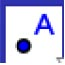
\includegraphics[scale=0.5]{images_geogebra/point.jpg}  & 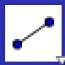
\includegraphics[scale=0.5]{images_geogebra/segment.jpg} \\ 
\hline 
Trace la droite perpendiculaire au segment [AB] et qui passe par le
point B. Puis tracer le cercle de centre B et qui passe par A. & 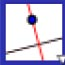
\includegraphics[scale=0.5]{images_geogebra/point_objet.jpg}  & 
\includegraphics[scale=0.5]{images_geogebra/cercle.jpg} \\ 
\hline 
Trace le point C, l'un des 2 points d'intersection du cercle et de la
droite. En faisant un clic droit sur le cercle, la droite et sur le second
point d'intersection, et en choisissant "afficher l'objet" tu les rendras
invisibles. Trace ensuite le segment [BC] & 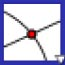
\includegraphics[scale=0.5]{images_geogebra/intersection.jpg}  & 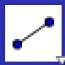
\includegraphics[scale=0.5]{images_geogebra/segment.jpg} \\ 
\hline 
Trace la droite perpendiculaire au segment [BC] et qui passe par le
point C. Puis tracer le cercle de centre C et qui passe par B. & 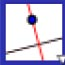
\includegraphics[scale=0.5]{images_geogebra/point_objet.jpg}  & 
\includegraphics[scale=0.5]{images_geogebra/cercle.jpg} \\ 
\hline 
Trace le point D, l'un des 2 points d'intersection du cercle et de la
droite. En faisant un clic droit sur le cercle, la droite et sur le second
point d'intersection, et en choisissant "afficher l'objet" tu les rendras
invisibles. Trace ensuite les segments [CD] et [DA] & 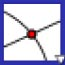
\includegraphics[scale=0.5]{images_geogebra/intersection.jpg}  & 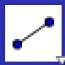
\includegraphics[scale=0.5]{images_geogebra/segment.jpg} \\ 
\hline 
Trace les points I, J, K et L, les milieux respectifs des segments [AB],
[BC], [CD] et [DA] & \multicolumn{2}{|>{\centering\arraybackslash}p{4cm}|}{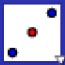
\includegraphics[scale=0.5]{images_geogebra/symetrie_centrale.jpg}}  \\ 
\hline 
\multicolumn{3}{|>{\centering\arraybackslash}p{14cm}|}{Mets tous les segments de la question précédente en rouge, et tous ceux formant le carré
en vert (pour cela fais un clic droit sur chaque segment, choisis l'option "propriétés",
puis l'onglet "couleur") } \\ 
\hline 
\end{tabular} 


